\section{Data Preparation}

\subsection{Cleaning the Dataset}
In this section, we are going to manipulate our dataset, in order to improve its quality and to facilitate the next analyses.

First of all, we focused on the \emph{NULL} values.\\
For what concerns the \textbf{CustomerID}, since our main goal is to outline the customer behavior, we decided to drop all the missing values for this attribute; therefore, we have eliminated \textbf{65073} rows.

\begin{comment}
Instead, regarding the \textbf{ProdDescr}, we can perform some data integration; in particular, we can fix these missing descriptions, gathering them from the other rows with the same \textbf{ProdID}.\\
In the first place, we need to remove the rows for which the \textbf{ProdID} appears just one time with \emph{NULL} description, since we cannot acquire any information about them from the data we have.\\
Now, we can integrate the remaining missing descriptions, getting them from the other objects in the dataset; from these operation, we were able to recover \textbf{768} rows.\\
From the data understanding regarding this attribute, we noticed some values that are not relevant for our analysis; so we decided to drop these rows, being particularly careful to not delete useful objects.
\end{comment}

Instead, regarding the \textbf{ProdDescr}, we notice that all the \emph{NULL} \textbf{ProdDescr} have also the \textbf{CustomerID} equal to \emph{NULL}; for that, we already eliminated these rows with the previous operation.\\ 
From the data understanding regarding this attribute, we noticed some values that are not relevant for our analysis; so we decided to drop these rows, being particularly careful to not delete useful objects.

Dealing with the \textbf{Sale} attribute, we can perform some kind of data integration.\\
In the dataset, we have \textbf{996} elements with a price equal to 0; that, of course, would represent a problem in the following phases of our work, since the information about the amount spent by a customer is crucial to understand its behavior. For that, we can correct those rows by extracting the informations we need from the rest of the dataset, checking by the \textbf{ProdID}. Here, we noticed that the price of a single product can show several variations, maybe due to the market fluctuations; we chose to take the mean of those values to integrate the rows in question.

About \textbf{BasketDate}, we decided to remove rows of the 2010, since the data were not taken regularly, and so they could alter our next study. On the contrary, we focus on the 2011 records, which were registered much more uniformly and are more useful and representative.

We also decided to delete the rows with a \emph{bad} \textbf{ProdID}, that we defined earlier as not a five digit code plus a variable number of characters. As a matter of fact, at this stage of data cleaning, the dataset contains only 4 unique \emph{bad} IDs, that are \emph{POST}, \emph{C2}, \emph{PADS} and \emph{DOT}; it is evident that they have an ambiguous meaning and so, they are not interesting in our context. As a result,we dropped \textbf{1273} elements.

We checked the attribute \textbf{CustomerCountry}, especially to see if some customer is associated to more than one country; in that case, we select, for each customer, the country registered with the most number of purchases.

\pagebreak
\begin{wrapfigure}{l}{.4\textwidth}
\centering
\captionsetup{justification=centering}
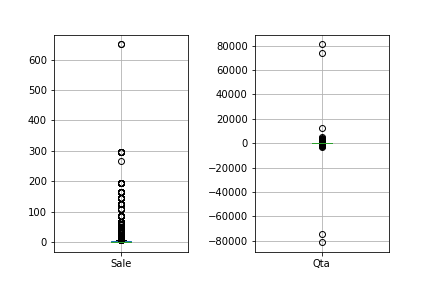
\includegraphics[width=0.39\textwidth]{img/boxplot_after.png}
\caption{Box plots\\ after the data cleaning}
\label{fig:boxplot_after}
\end{wrapfigure}

We also looked at the outliers we already detected with the box plots in the previous section.\\
As we can see in Figure \ref{fig:boxplot_after}, the previous operations already cleaned some of the outliers we had in the original dataset; now we manually check them, to determine if they are errors or not.\\
In the case of \textbf{Sale}, we have that the maximum value is 649.5, which is quite high; in reality, we discovered that all the outliers for this attribute are referring to purchases of furniture or objects sold in big quantities, \emph{e.g.} 60 picnic baskets. So we consider these rows as correct.\\
In the case of \textbf{Qta}, we see just two values that are really away from the others, and they represent huge purchases, with quantities equal to 74251 and 80995; we have also the same quantities in negative. Since this is a very strange case, we thought that they could be the results of an error and so we decided to drop these 4 rows.

We ended up with a cleaned dataset, consisting of \textbf{373364} entries.

\begin{figure}[h!]
\captionsetup{justification=centering}
\begin{subfigure}{.3\textwidth}
\centering
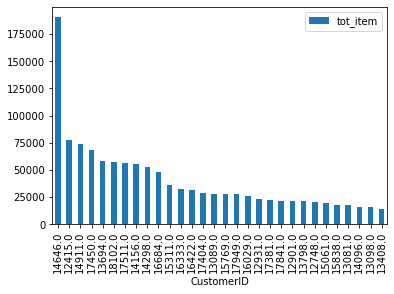
\includegraphics[width=\textwidth]{img/tot_item.png}
\caption{Total number of items per customer}
\label{fig:tot_item}
\end{subfigure}
\begin{subfigure}{.3\textwidth}
\centering
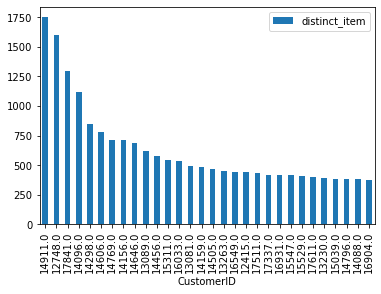
\includegraphics[width=\textwidth]{img/distinct_item.png}
\caption{Number of distinct items per customer}
\label{ref:distinct_item}
\end{subfigure}
\begin{subfigure}{.3\textwidth}
\centering
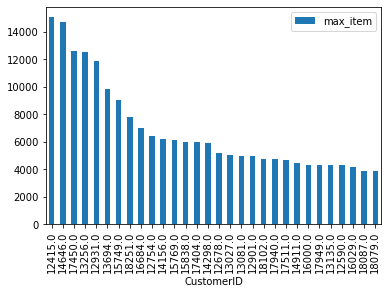
\includegraphics[width=\textwidth]{img/max_item.png}
\caption{Maximum number of items per customer}
\label{fig:max_item}
\end{subfigure}
\caption{Visualization for the extracted features}
\label{fig:first_features}
\end{figure}

\subsection{Feature extraction}
Here, we extract new features from the dataset, in order to describe the customers behavior.\\
First of all, we defined some basic features, like:
\begin{itemize}
\item The total number of items purchased by a customer
\item The number of distinct items bought by a customer
\item The maximum number of items purchased by a customer during a shopping session
\end{itemize}

In Figure \ref{fig:first_features}, we can see some visualization for the features we just extracted; in particular, they represent the first 30 customers with the biggest values for each feature.\\
An interesting information is clear from the plot \ref{fig:max_item}, where we can see that the maximum quantities purchased in a single shopping session are very big; they are all above 3500, with the maximum equal to 15049. These are very high values, unlikely for a retail customer; this led us to think that the supermarket in question also sells wholesale.

\begin{wrapfigure}{l}{.5\textwidth}
\centering
\captionsetup{justification=centering}
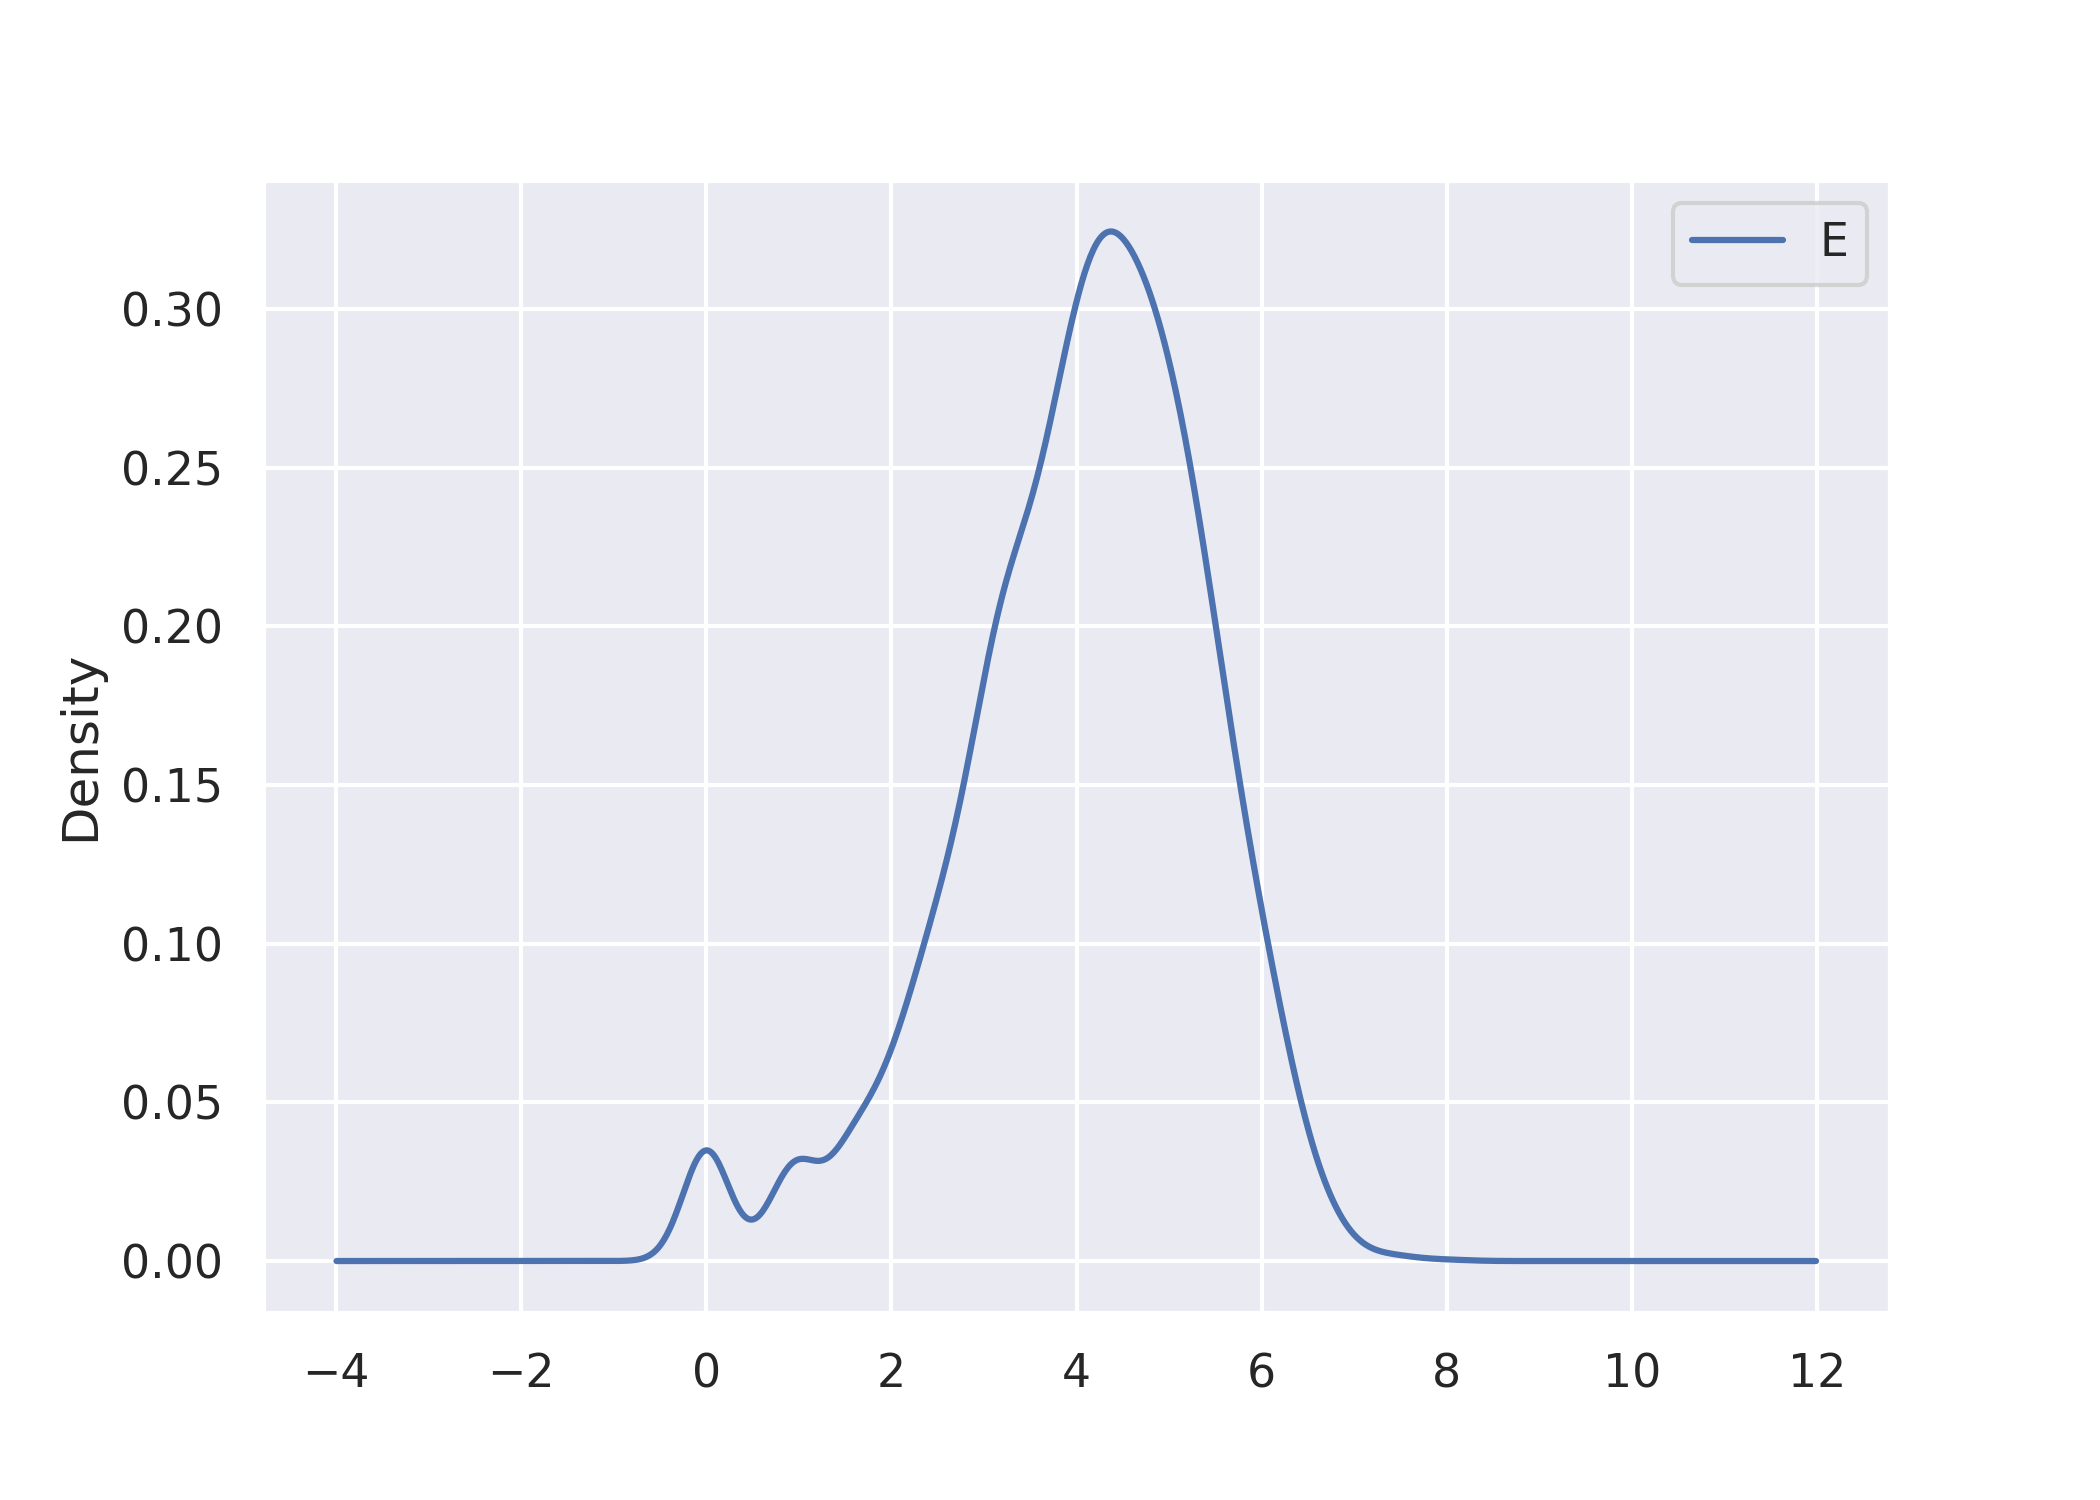
\includegraphics[width=0.49\textwidth]{img/kde_entropy.png}
\caption{Entropy distribution}
\label{fig:kde_entropy}
\end{wrapfigure}

\begin{comment}
To compute the entropy we defined two categorical attributes which are the result of the discretization of \textbf{Qta} and \textbf{TotPrice}. The attribute \textbf{Qta} was discretized by observing that $\sim 18\%$ of the rows have \textbf{Qta} equals to one, so we introduced the category \emph{Single}. Other than that we created also the categories \emph{Small}  (from $2$ to $6$), \emph{Medium} (from $7$ to $12$), \emph{High} (from $12$ to $36$) and \emph{Very High} (larger than $37$). For what concern the category related to \textbf{TotalPrice} we set an equal frequency binning into five categories. The entropies, \textbf{QtaEntr} and \textbf{TPEntr}, measure the variability of the customer's spending and quantity habit.
\end{comment}

In Figure \ref{fig:kde_entropy}, we can evaluate the distribution of the entropy. In particular, we are focusing on the attribute \textbf{TotalPrice}.
This value of the entropy represents the variability of the customer's spending habits; a bigger value means that the customer did not have a regular behavior, instead he spent always different amount of money.\\
We have a small peak corresponding to 0, meaning that there are some customers with very specific habits, but the maximum is reached for $\sim 4$, which means that the majority of the clients have a quite unpredictable behavior.

Since the focus is on the purchasing behavior of the customers, we decided to study other features, in order to deeply understand the information we have. We chose to extract information about:
\begin{itemize}
\item The number of basket per customer
\item The number of \emph{bad} basket per customer
\item The number of purchased products
\item The number of returned products
\item The amount of money spent for each customer
\item The amount of money refunded per customer
\end{itemize}

Thanks to these features, we were able to see better the kind of customers registered in the dataset.\\
First, we checked if there were customers with a number of returned products bigger than the purchased ones; as a matter of fact, we found \textbf{18} rows of this kind. We consider these as \emph{bad} customers, since they have made more returns than purchases; this is clearly an impossible situation, maybe due to the fact that some transaction was not registered in the dataset.
Anyway, we decided to delete these customers.\\
Plus, we inserted two other columns:
\begin{itemize}
\item \textbf{ActualQta}, which is the algebraic sum between the positive and the negative quantities
\item \textbf{ActualSpent}, equal to the difference between the money spent and the one refunded
\end{itemize}

We also deleted all the customers with the \textbf{ActualQta} equal to zero, since, in the end, they didn't buy anything. 

Now we extract some information about the average values, as:
\begin{itemize}
\item \textbf{AvgPrice}, the ratio between \textbf{ActualSpent} and \textbf{ActualQta}, that represents the average price of the products bought by a customer
\item \textbf{AvgBaskValue}, the ratio between \textbf{ActualSpent} and the number of \emph{good} baskets, which represents the average amount of money spent for each basket per customer
\end{itemize}

\begin{wrapfigure}[13]{r}{.5\textwidth}
\centering
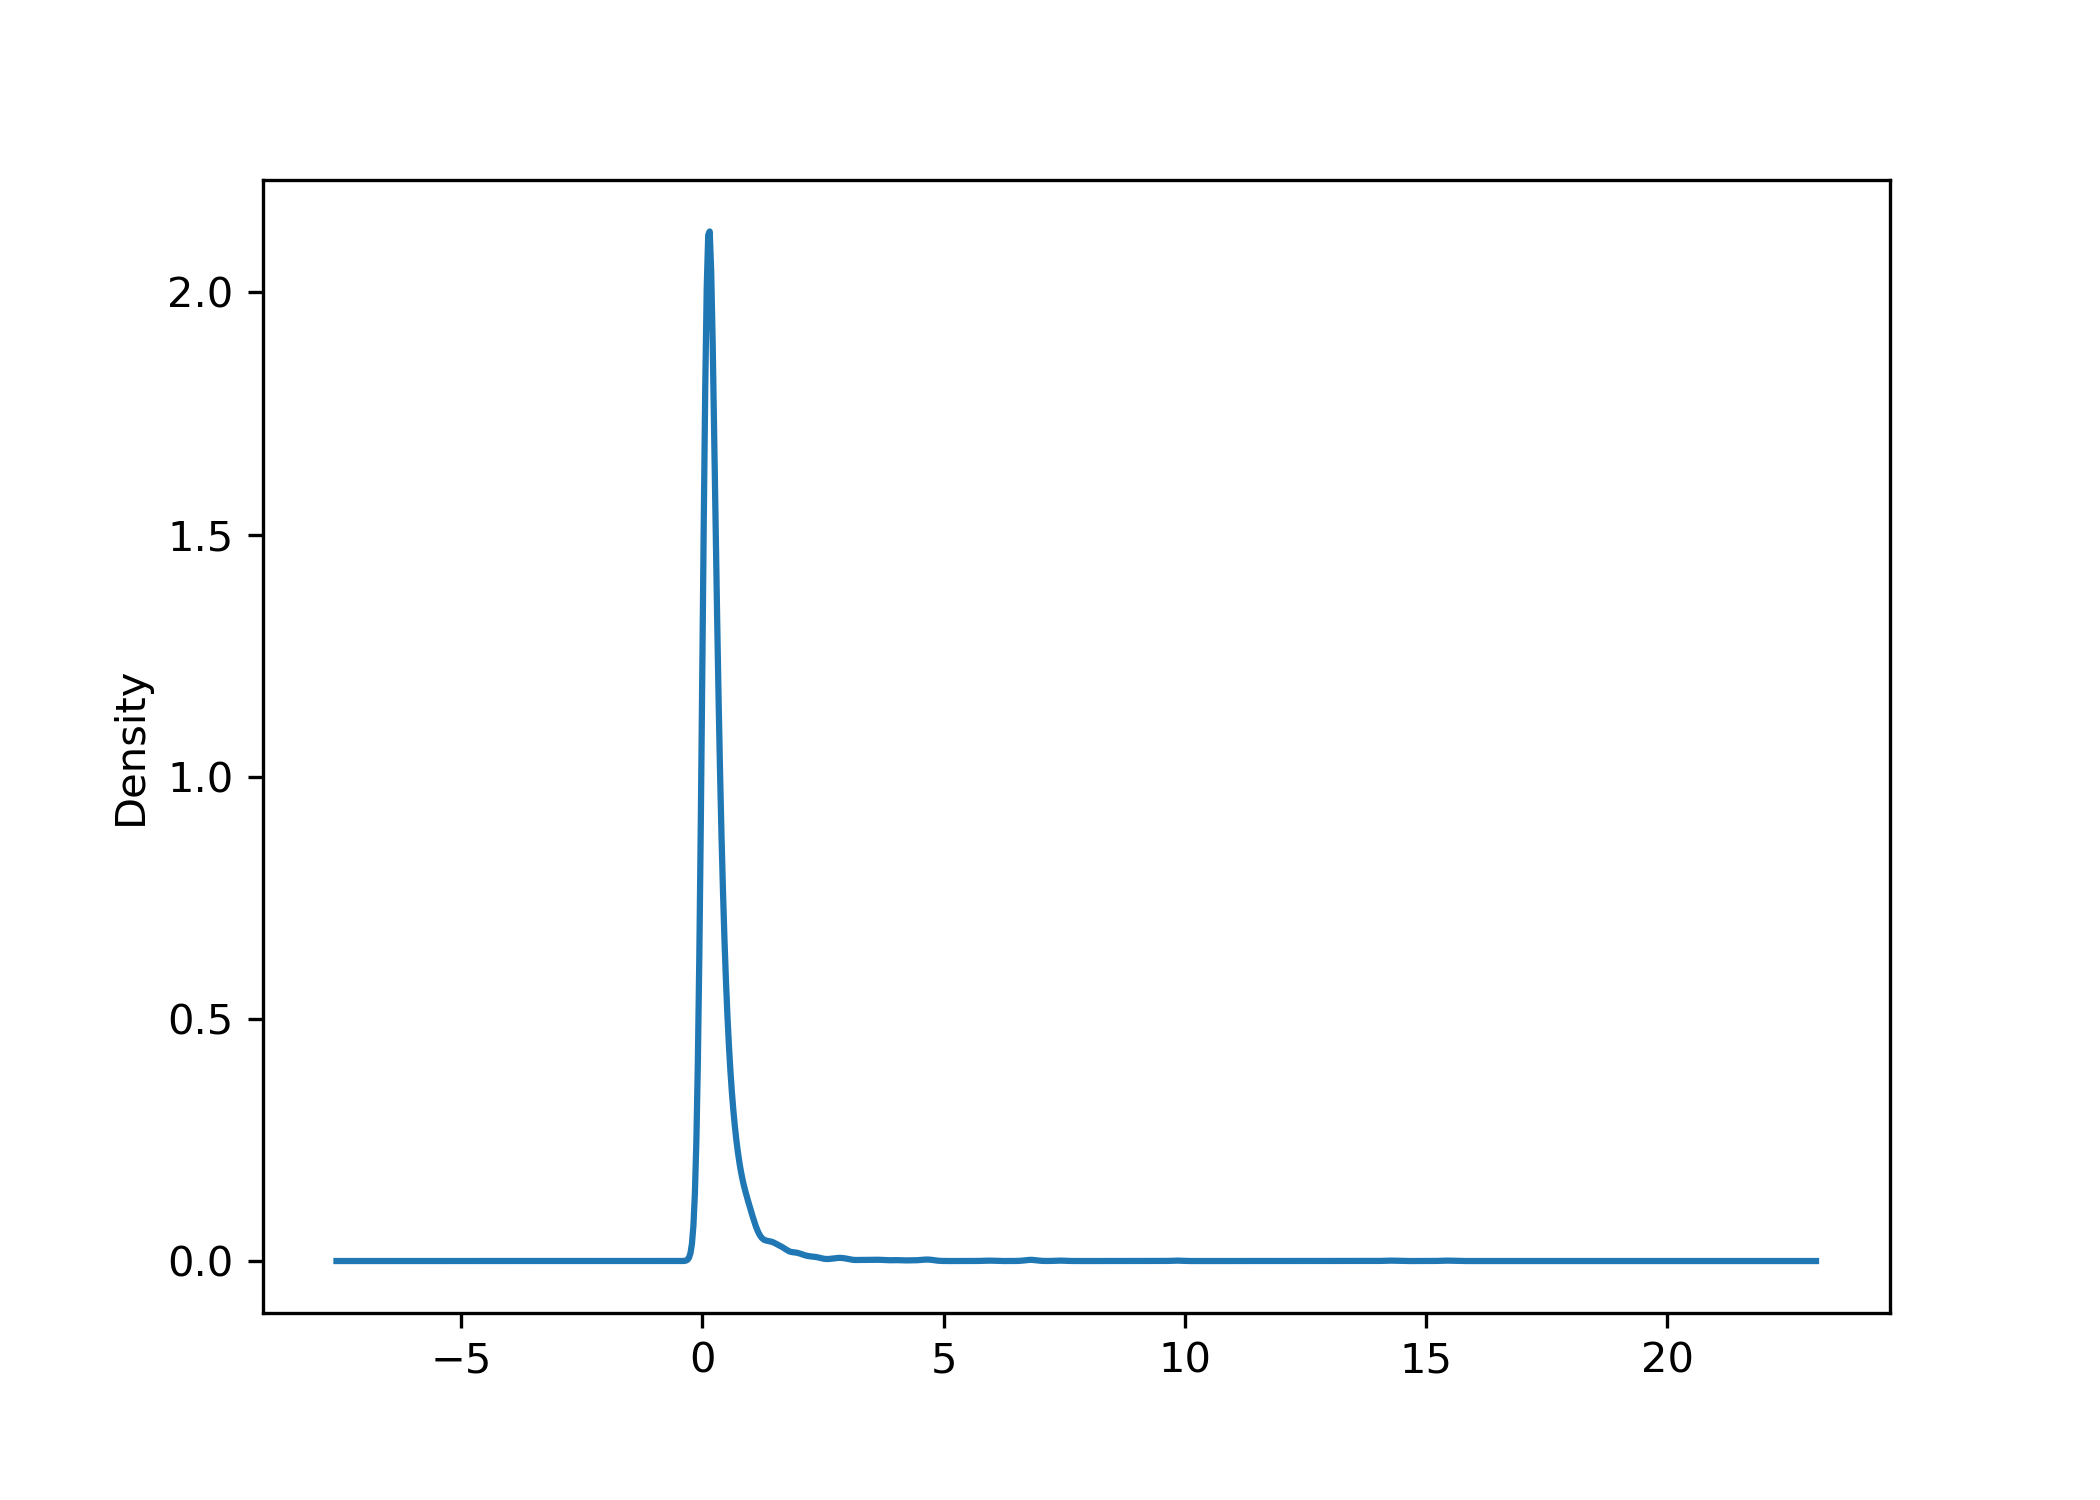
\includegraphics[width=0.49\textwidth]{img/monthfreq.png}
\caption{Monthly Frequency}
\label{fig:month_freq}
\end{wrapfigure}

Another interesting feature is the \textbf{MonthFreq}, that we computed as the ratio between the number of \emph{good} baskets and 12, the number of months. We can visualize this attribute in the Figure \ref{fig:month_freq}, where we can clearly see that the peak is really close to 0; in fact, the mode of this column in equal to \textbf{0.083}, which means that the majority of the customers went to this supermarket just once in the year.

\begin{figure}
\captionsetup{justification=centering}
\begin{subfigure}{0.5\textwidth}
\centering
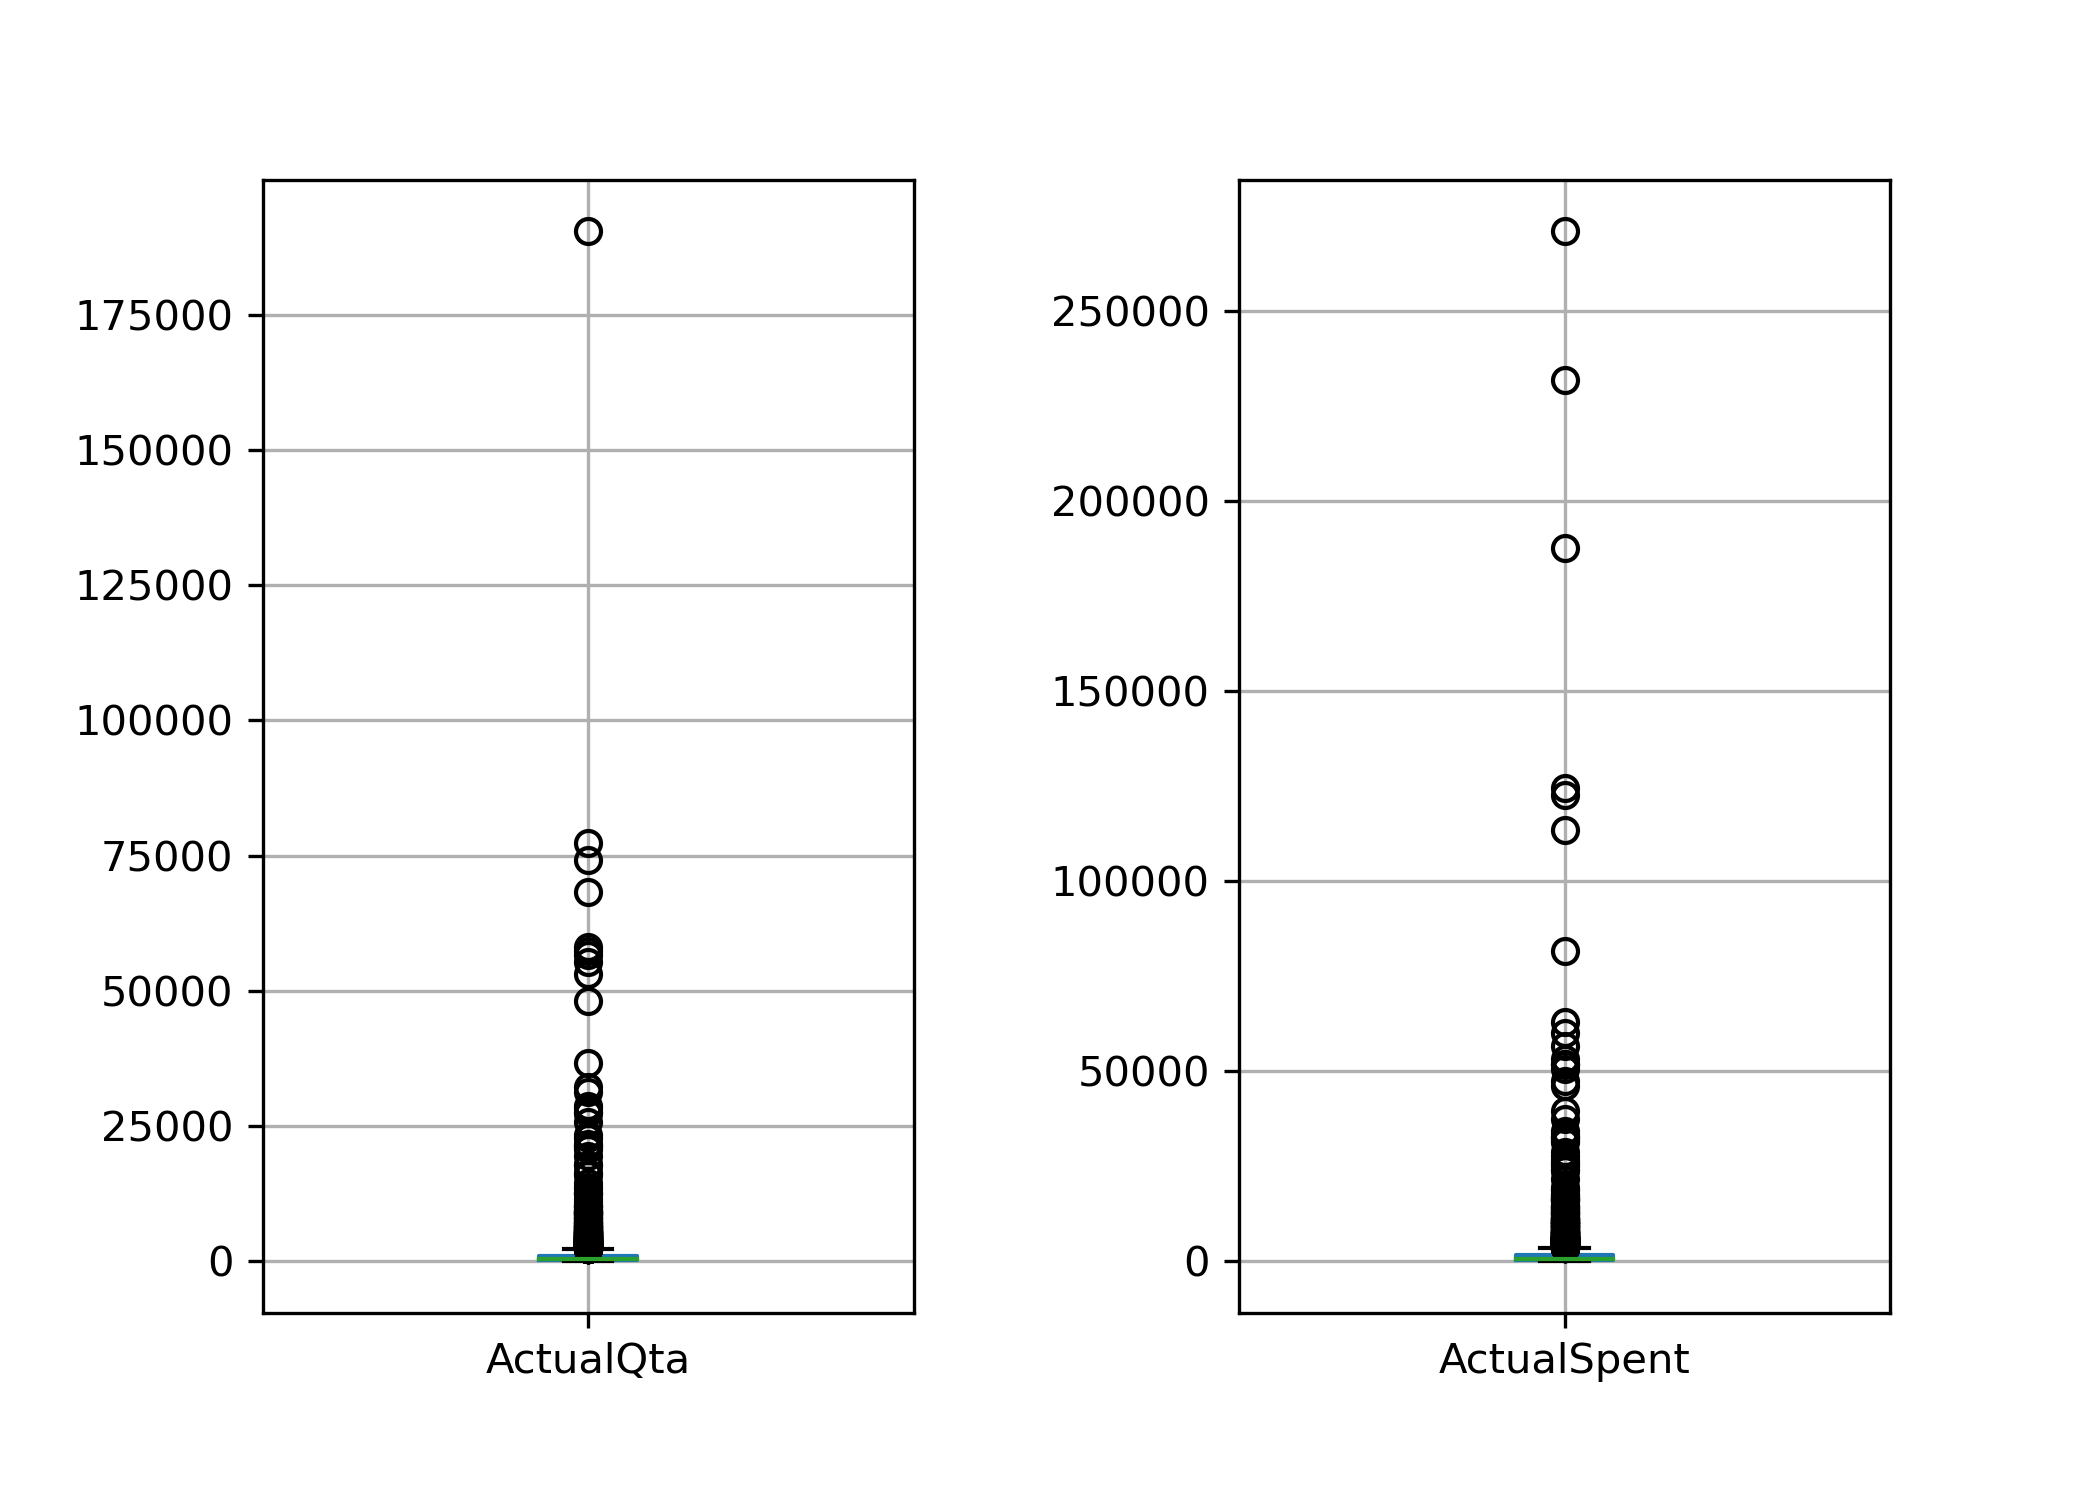
\includegraphics[width=\textwidth]{img/boxplot_for_actuals.png}
\caption{}
\label{fig:boxplot_actuals}
\end{subfigure}
\begin{subfigure}{0.5\textwidth}
\centering
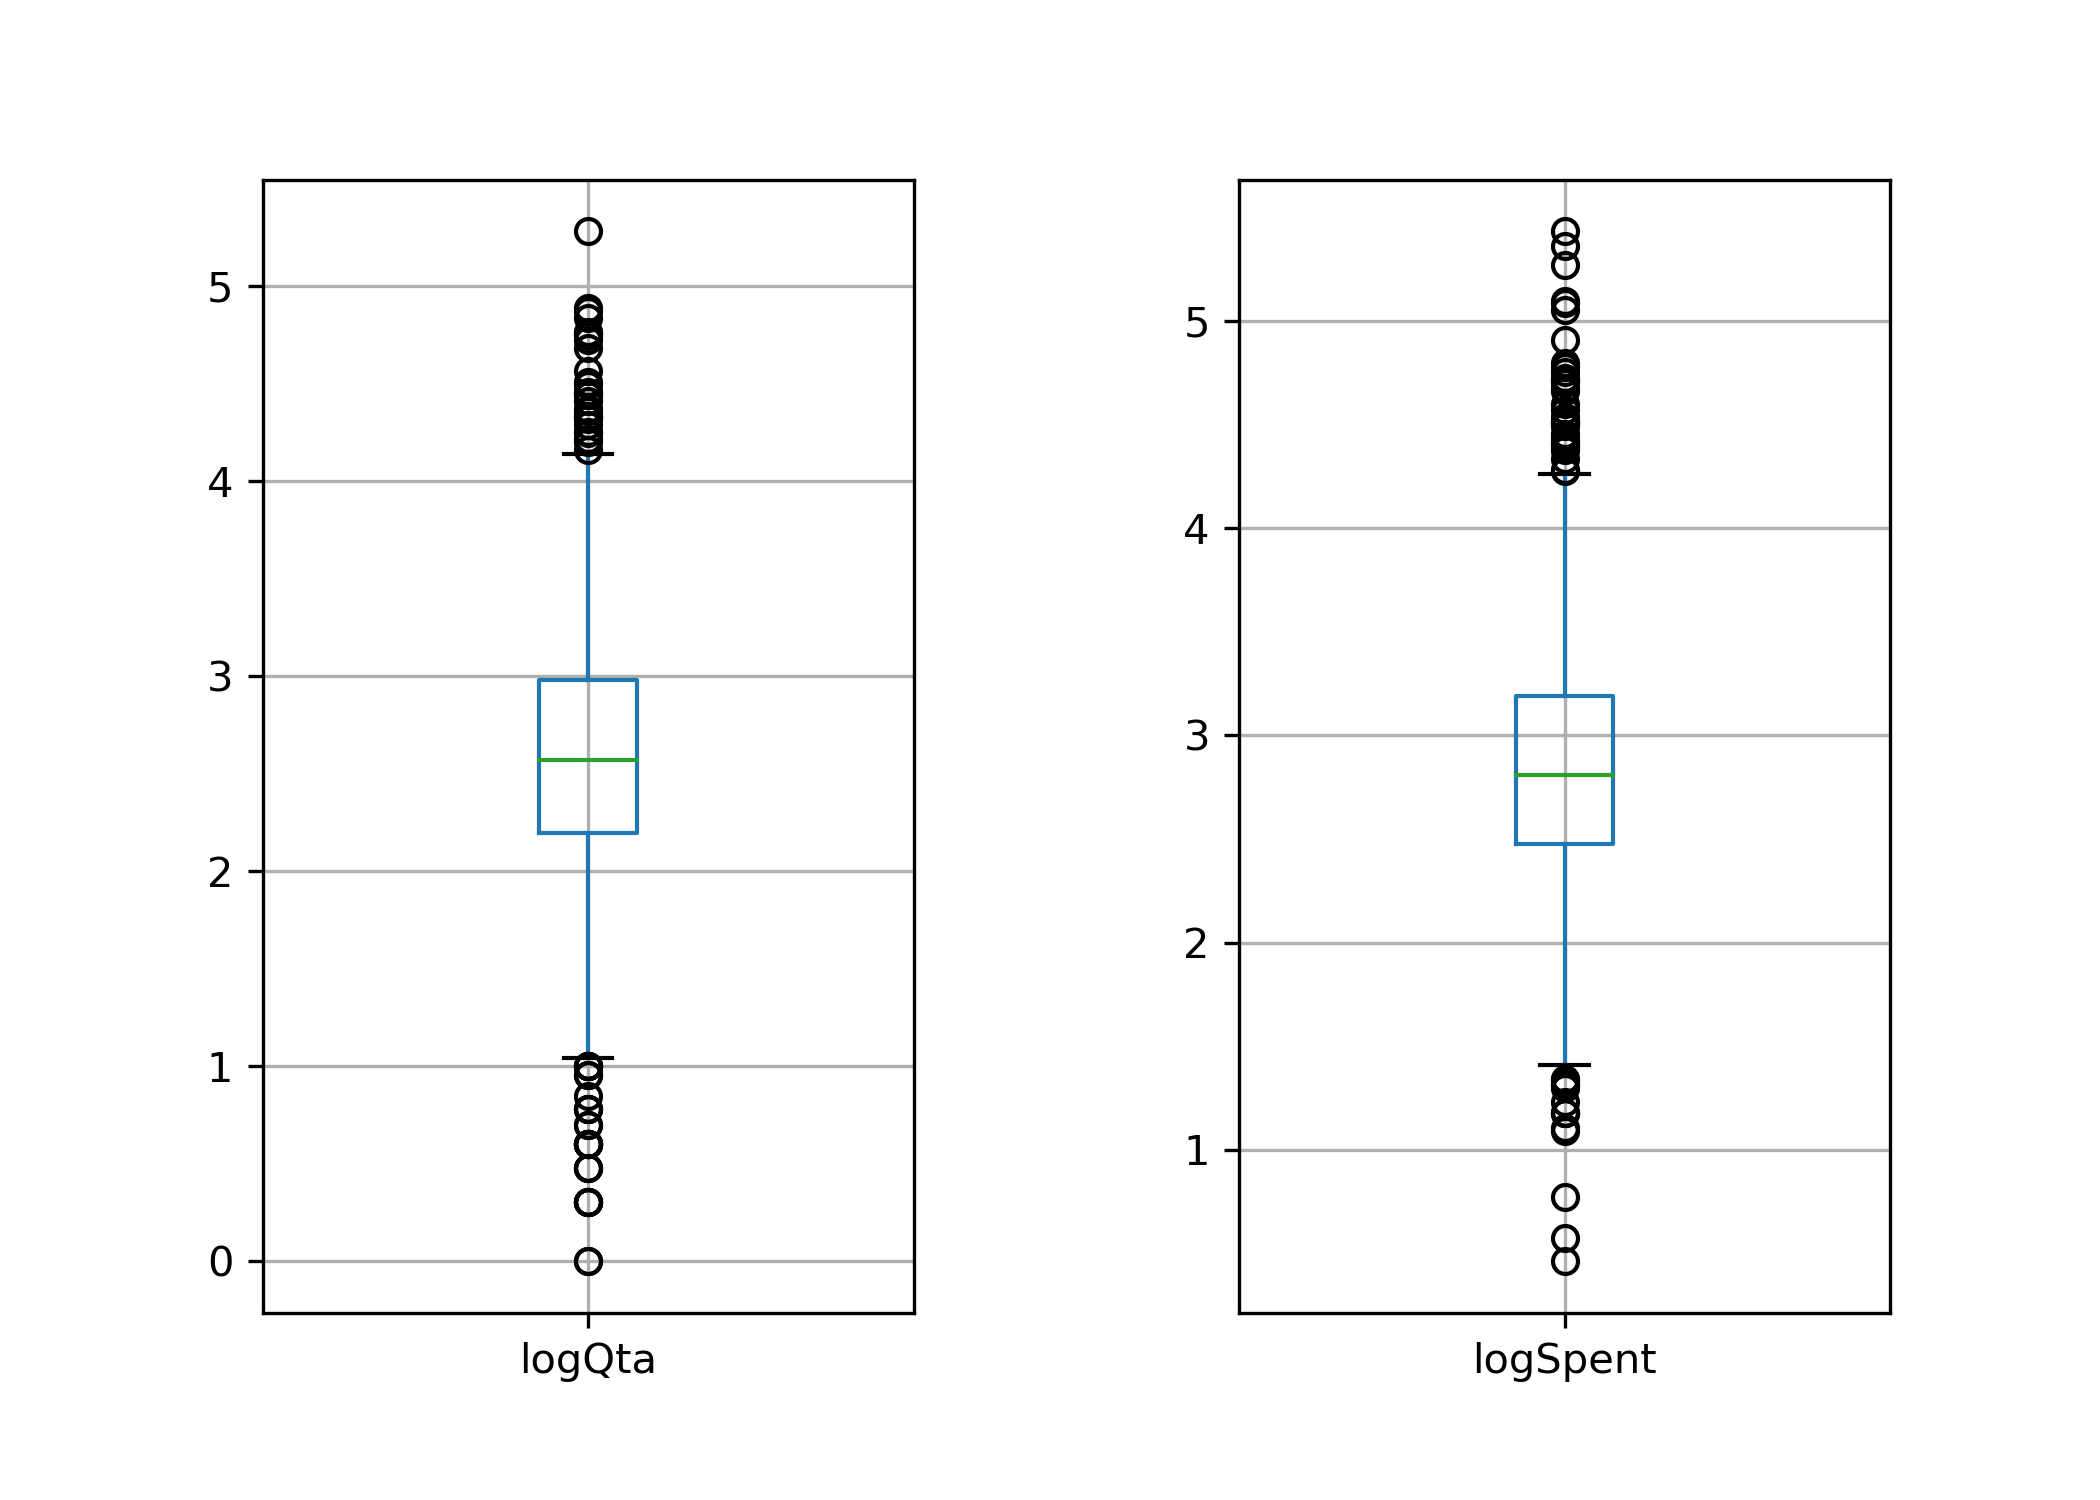
\includegraphics[width=\textwidth]{img/boxplot_for_log_actuals.png}
\caption{}
\label{fig:boxplot_logs}
\end{subfigure}
\caption{Box plots for ActualQta and ActualSpent, before and after the log}
\end{figure}

Analyzing the Figure \ref{fig:boxplot_actuals}, we can see that the attributes \textbf{ActualQta} and \textbf{ActualSpent} are really spread; for this reason, we consider their logarithm in base 10, so that the difference between high values has a different weight. We can appreciate the changes in the Figure \ref{fig:boxplot_logs}, where the two distributions are much more compact.\\
After the transformations of these attributes, we saw that also \textbf{AvgPrice} and \textbf{AvgBaskValue} were quite spread, and so we decided to compute the same operation to them.

\pagebreak

\begin{wrapfigure}[12]{l}{0.5\textwidth}
\centering
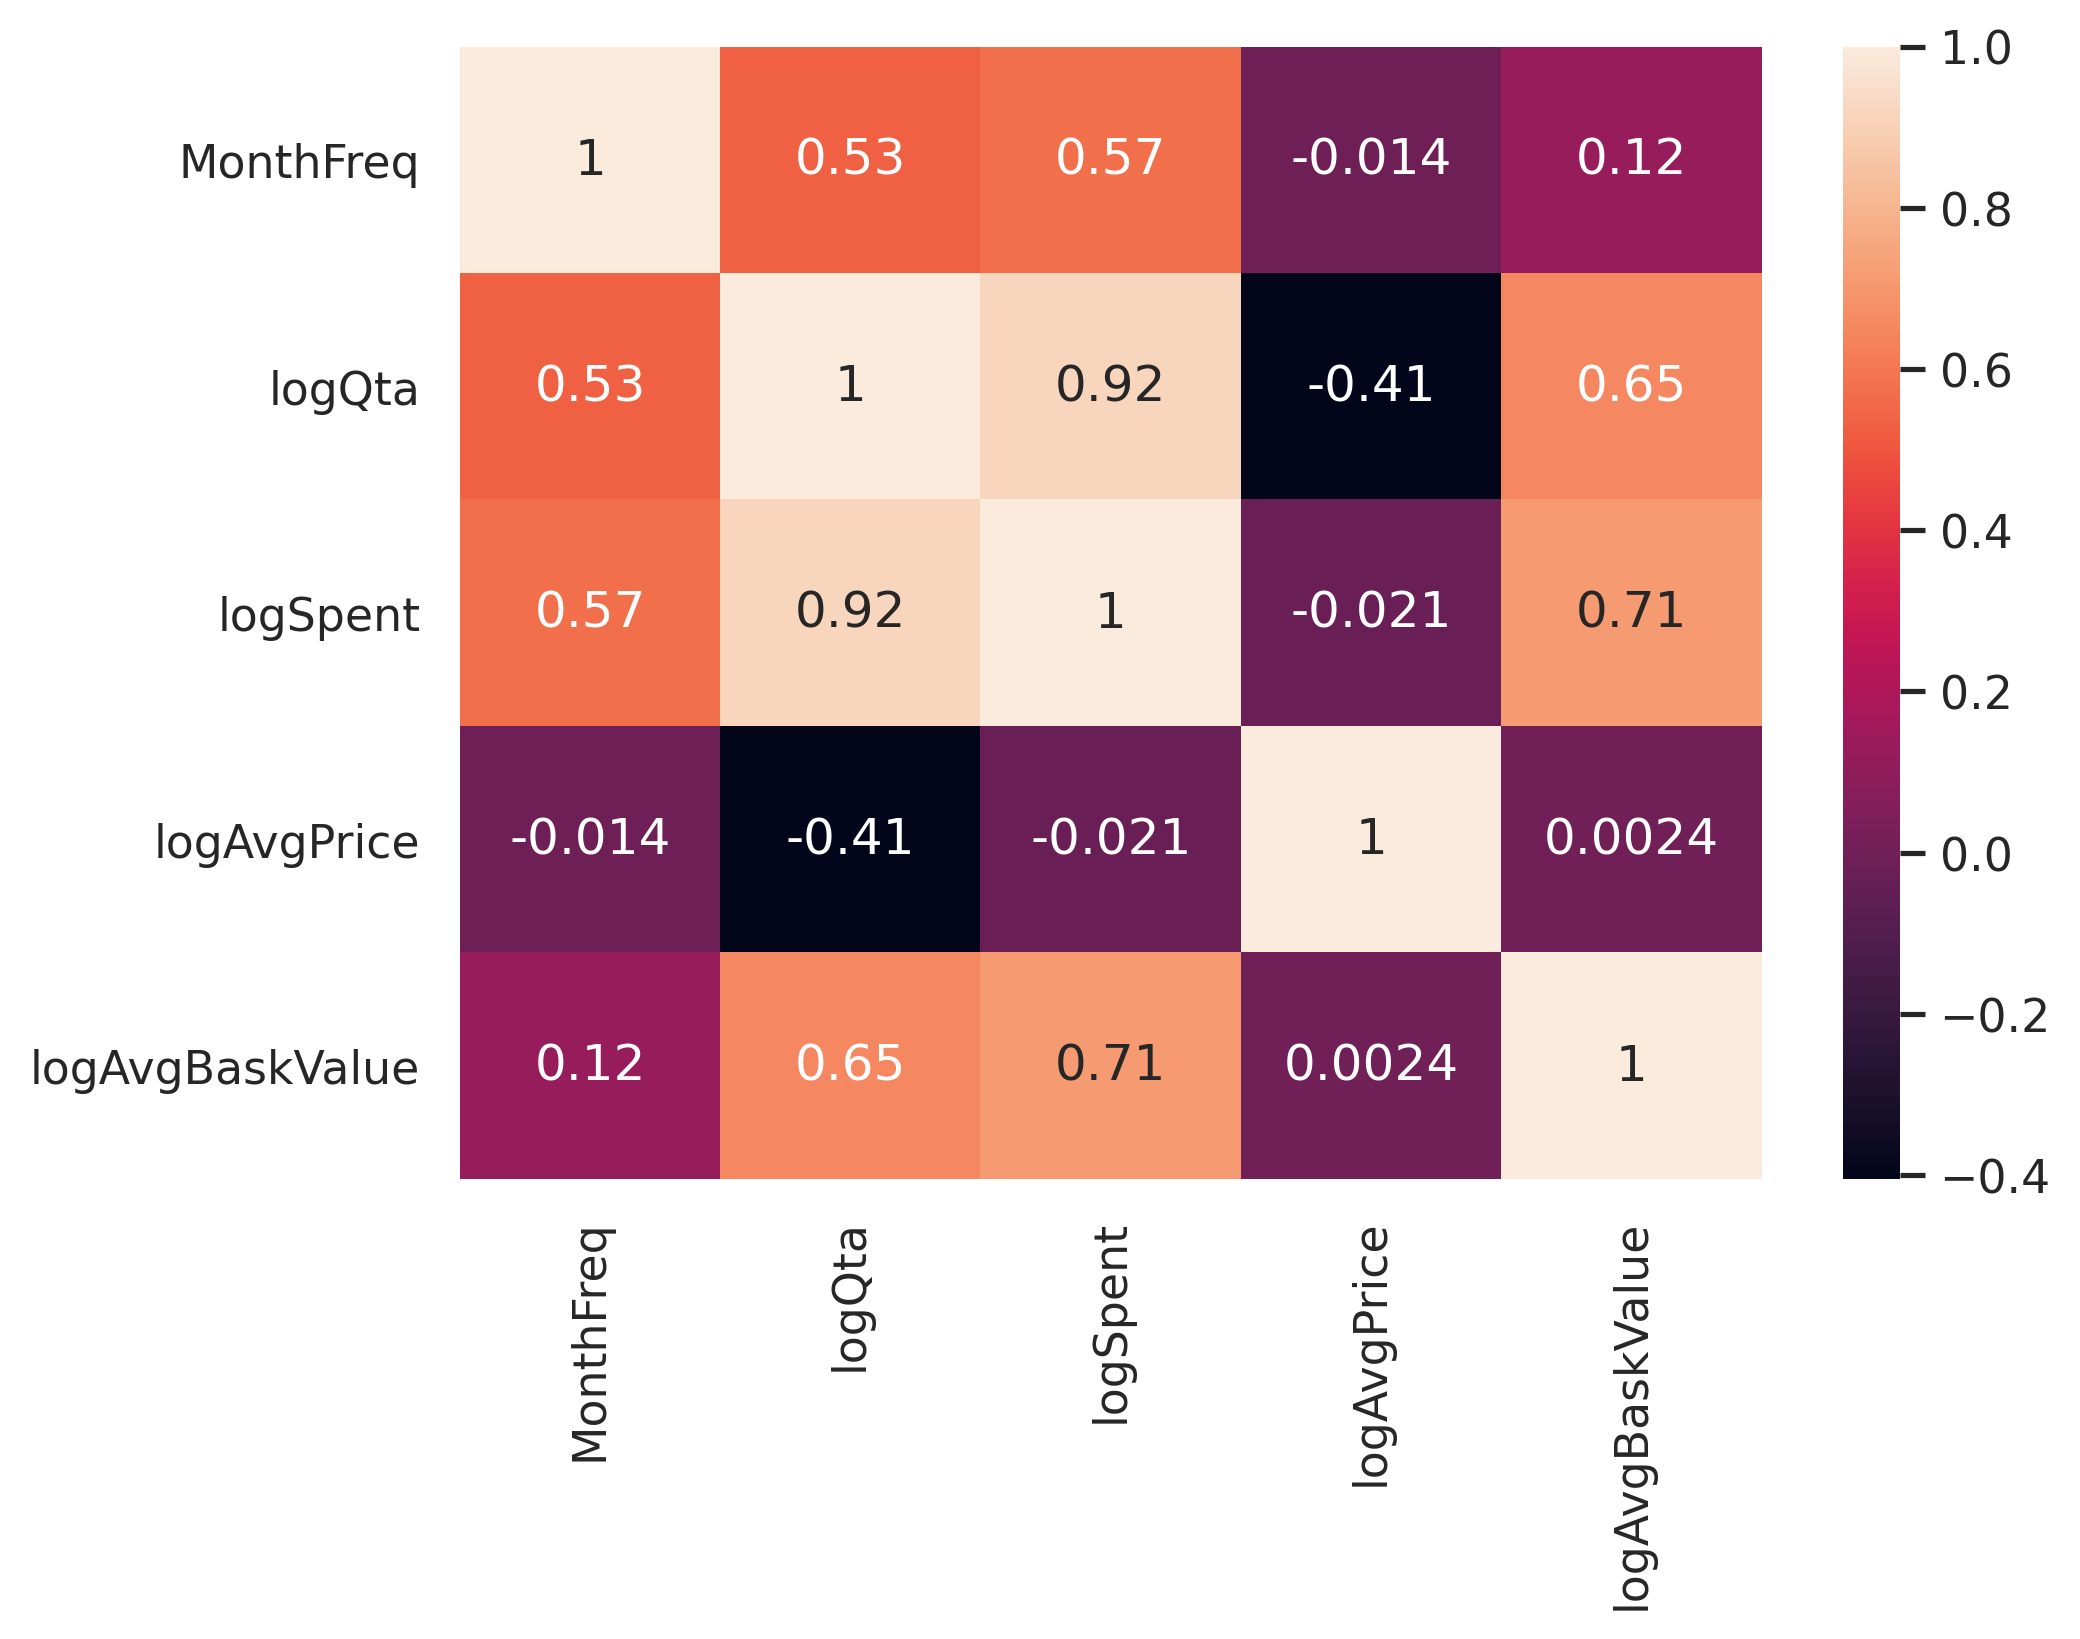
\includegraphics[width=0.49\textwidth]{img/corr_logs.png}
\caption{Correlation Matrix}
\label{fig:corr_logs}
\end{wrapfigure}

Now, we can visualize the correlation between the attributes. In Figure \ref{fig:corr_logs}, as expected, we find that the average basket value is highly correlated with the total quantity purchased and the amount of money spent. Furthermore, we can see that also the monthly frequency is correlated with the amount spent and the total quantity. In the end, of course, the quantity purchased is very highly correlated with the total amount spent.

\vspace{10mm}

\begin{wrapfigure}{r}{0.45\textwidth}
\centering
\captionsetup{justification=centering}
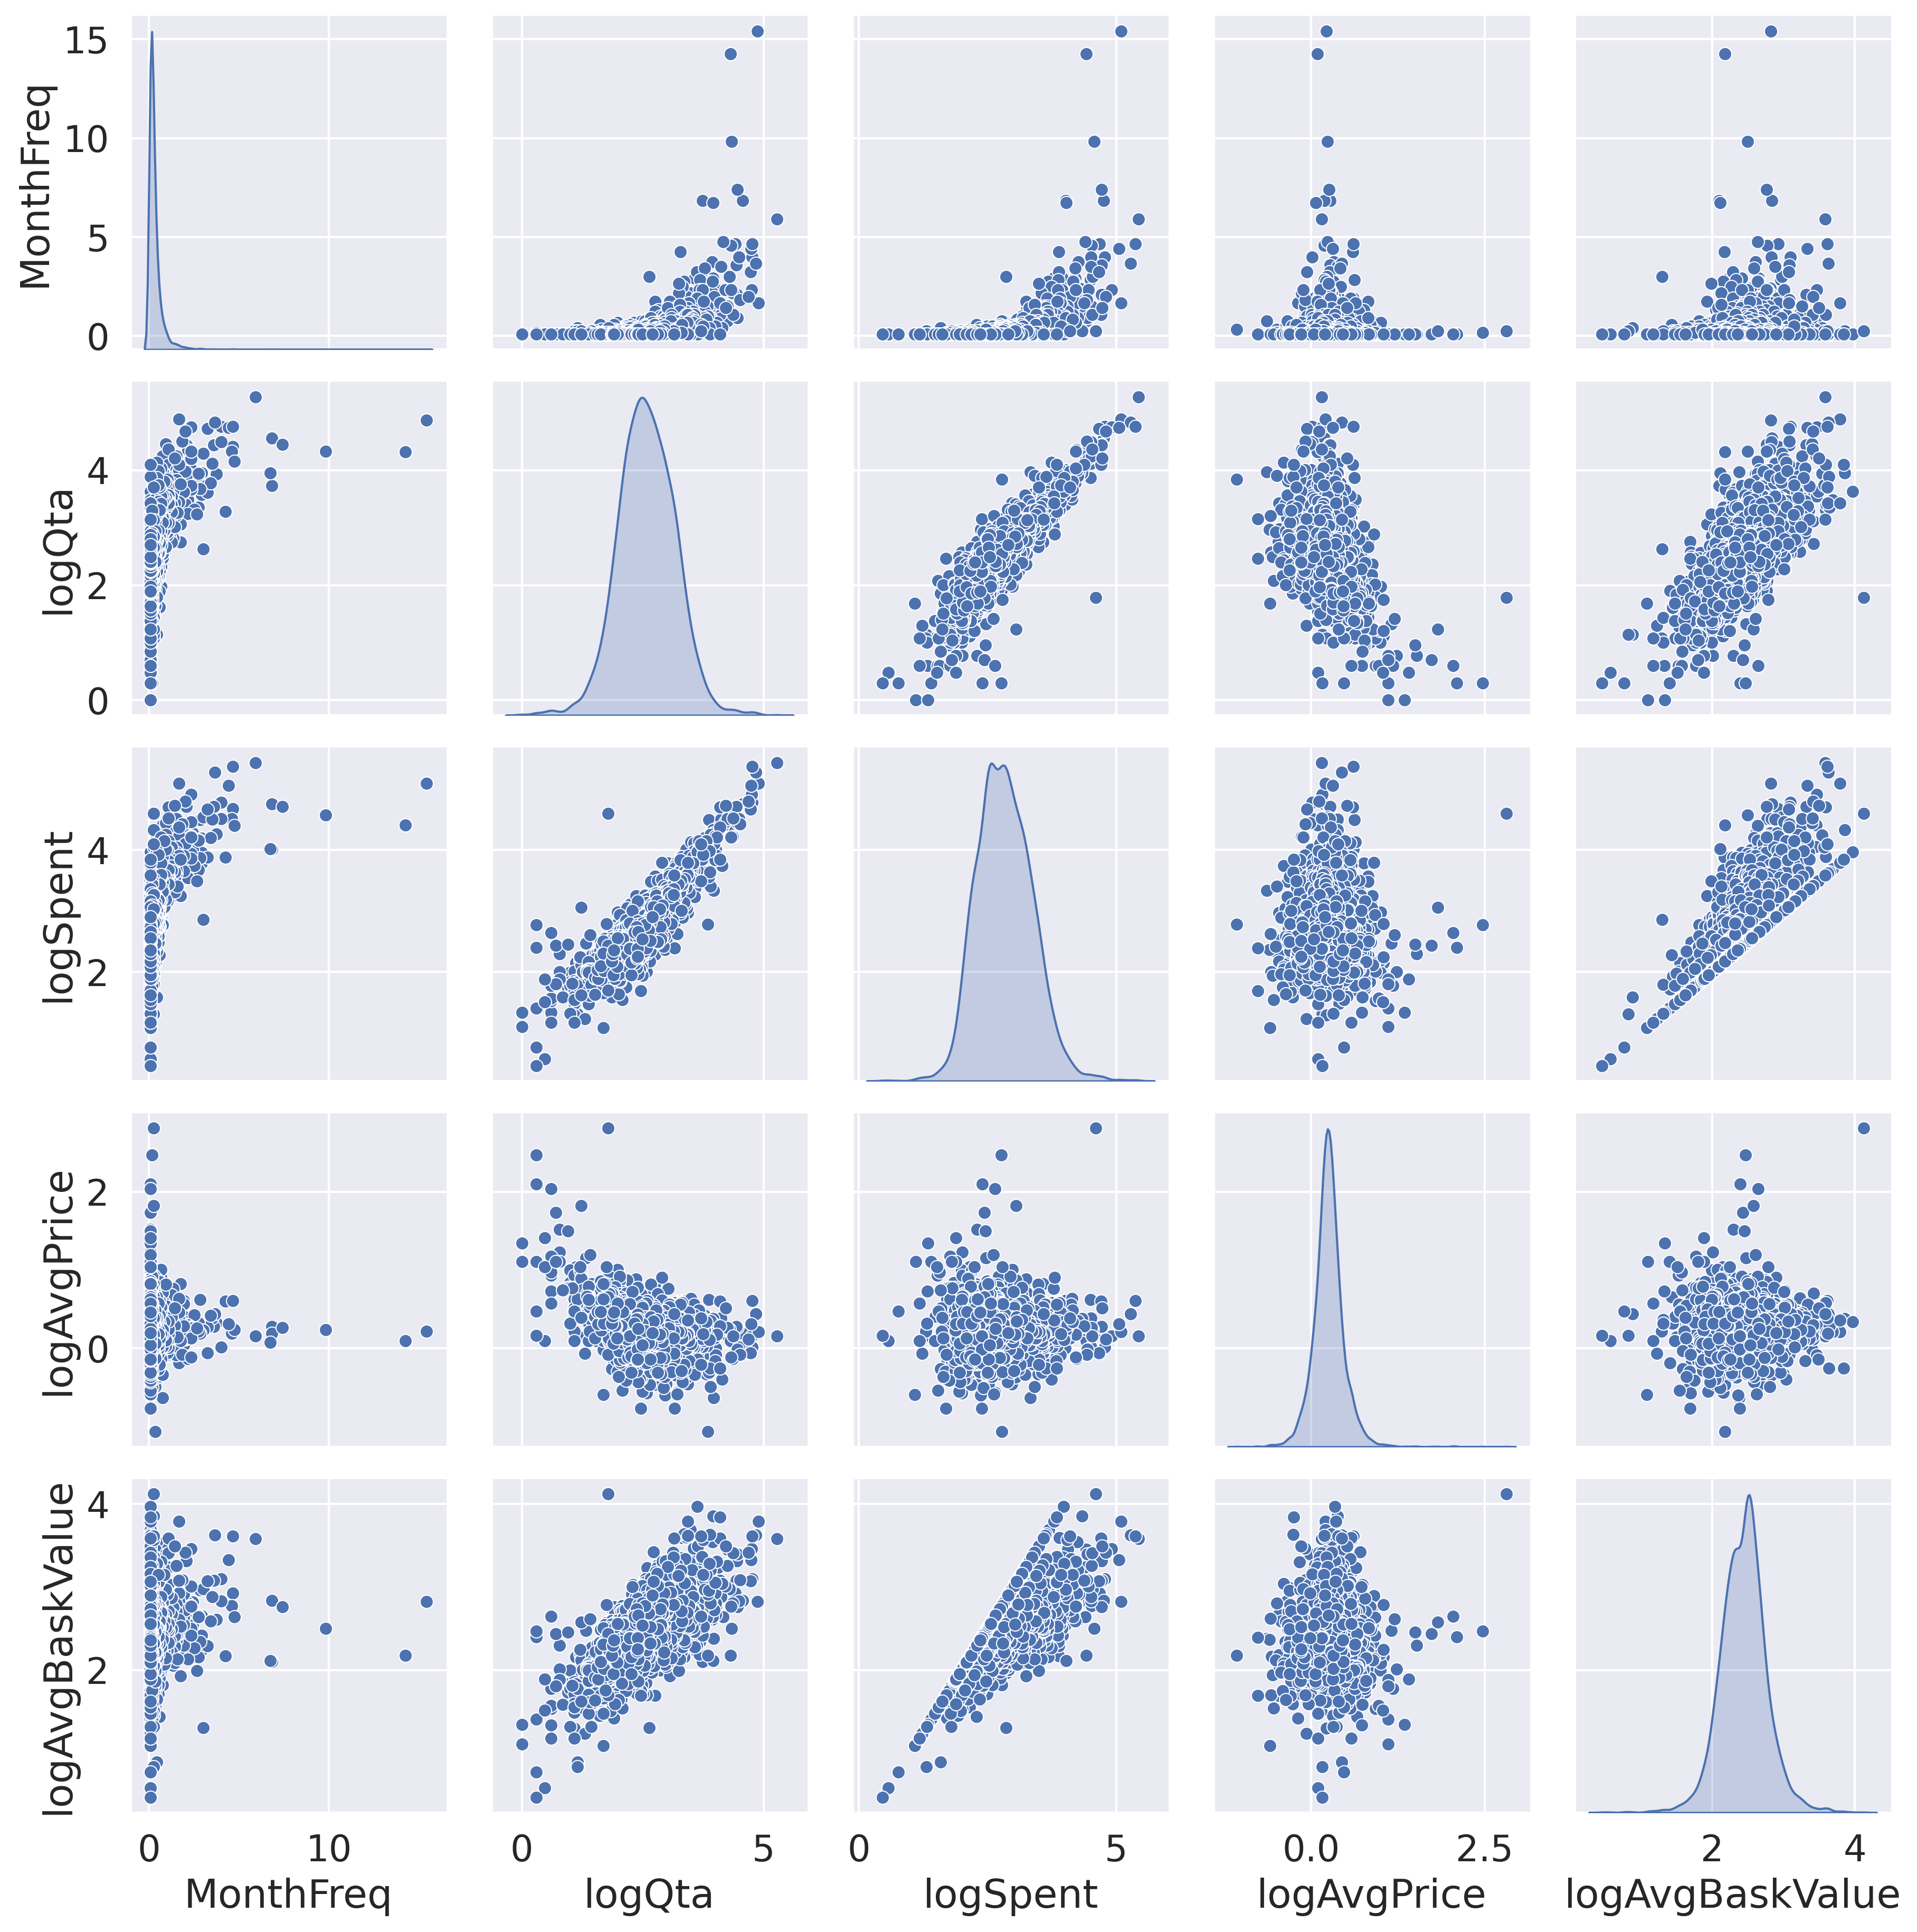
\includegraphics[width=.44\textwidth]{img/pairplot.png}
\caption{Pair Plots}
\label{fig:pairplot}
\end{wrapfigure}

In Figure \ref{fig:pairplot}, we can visualize the Pair Plot for the attributes we have.\\
On the diagonal, we have the density plots, where we can appreciate the distribution of the features. Instead, the other scatter plots show the relationship between two variables. By analyzing those, we can have a confirmation of what we already found thanks to the previous plot. 

\begin{comment}
\begin{figure}[h!]
\centering
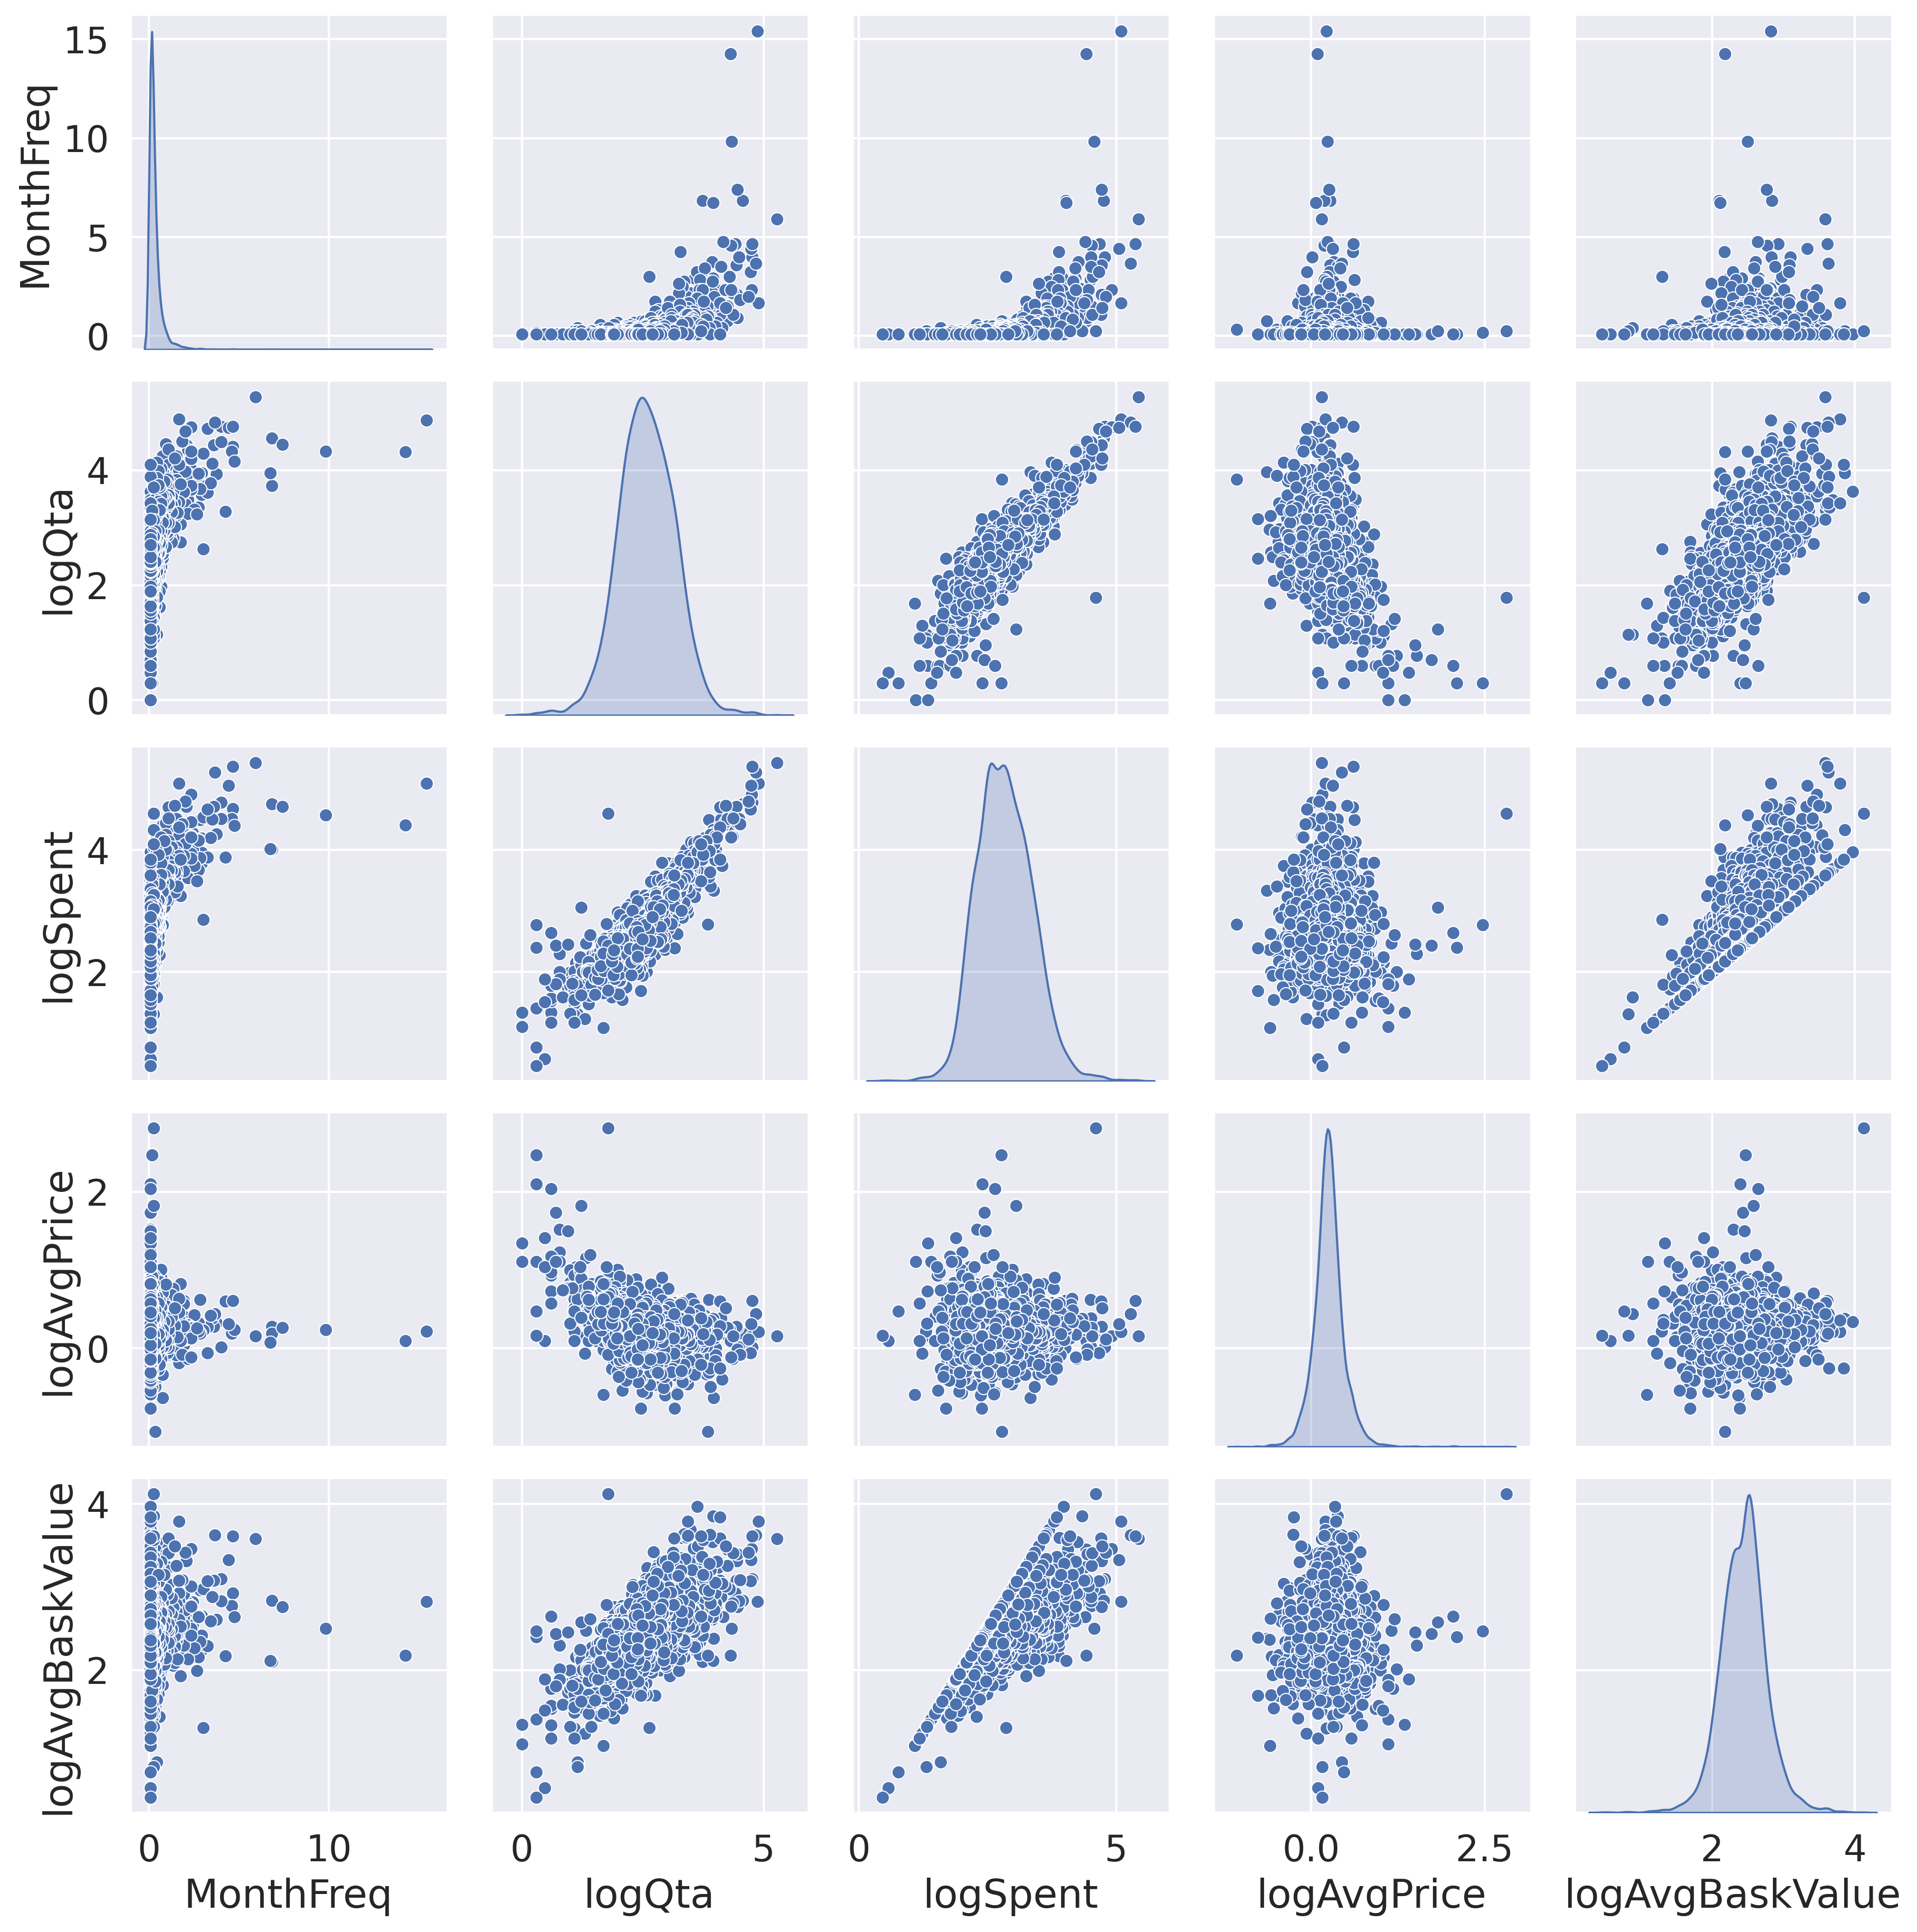
\includegraphics[width=.5\textwidth]{img/pairplot.png}
\caption{Pair Plots}
\label{fig:pairplot}
\end{figure}
\end{comment}
